\chapter{第三章 总体架构设计}
\section{系统设计目标}
\subsection{高保真性}
高保真性是本系统的核心目标之一,要求生成的交通场景能够最大限度地忠实反映自然语言描述。为了实现这一目标,系统不仅需要保证场景的视觉效果和语义的一致性,还应考虑各种复杂的环境要素和交通行为的准确性。例如,生成的场景中各类交通工具的行为需要与现实世界中的交通流动一致,交通规则和行为模式需要严格遵循。因此,系统需要通过对输入描述进行精确解析,使用先进的自然语言处理技术(如大语言模型)来理解场景中的各种细节,并转换为对应的三维仿真环境。这些细节不仅仅是物理上的位置和对象,更包括交通元素之间的动态互动,环境条件如天气、时间、光照等因素的考虑。

\subsection{自动化}
自动化是本系统设计的另一个关键目标。通过实现从自然语言输入到场景生成与仿真运行的自动化流程,系统能够减少人工干预,提高效率并降低人为错误的发生。系统应能够通过少量的用户输入(例如一段简短的自然语言描述)完成从场景构建到仿真运行的全过程,自动生成所有必要的配置文件,调度仿真平台执行,并收集仿真结果进行后续分析。自动化不仅限于场景生成,也包括场景的评估和结果展示,能够在生成后直接对场景进行可视化、量化评估,并输出最终报告。这种全自动的流程将极大地提升仿真研究的效率,支持大规模的实验和多样化的场景生成需求。

\subsection{可扩展性}
可扩展性是系统设计中的重要原则,确保系统能够随着需求的变化进行功能和技术的扩展。系统设计应当采用模块化的结构,每个功能模块(如自然语言处理、场景生成、仿真执行、评估展示等)都可以独立发展和优化,并与其他模块无缝衔接。可扩展性体现在以下几个方面:
\begin{itemize}
	\item 自然语言处理模型的升级:随着自然语言处理技术的发展,新的语言模型和算法可能会不断出现,系统应当能够灵活集成新的语言模型,提升场景生成的准确性和多样性。
	\item 仿真平台的集成:虽然当前平台使用CARLA作为仿真引擎,未来可能会考虑集成其他仿真平台或与不同的驾驶仿真系统对接,以支持更多元的实验需求和不同平台的比较。
	\item 评估指标的多样性:系统的评估模块应支持定制化和多维度的评估指标,未来可以根据不同的场景类型、研究需求或应用场景,添加新的评估标准,改进现有评估方法。
\end{itemize}

\subsection{核心功能实现}
本系统的核心功能涵盖三个关键方面:
\begin{itemize}
	\item 从自然语言描述中自动生成三维交通场景:这一功能是系统的基础,旨在通过对输入的自然语言进行理解,自动生成能够在仿真环境中运行的交通场景。系统将利用自然语言处理模型和检索增强技术,结合已有的场景模板和元素库,实现语义精确的场景建模。
	\item 对生成的场景进行仿真与可视化:该功能主要确保生成的三维场景能够在仿真平台中正确呈现并运行。系统通过调用仿真平台API,自动将生成的场景描述转化为可执行的仿真环境,并进行实时仿真与动态可视化。此过程还包括对场景中交通元素的行为模拟,例如交通流、车辆行驶轨迹、交互等。
	\item 对生成结果进行量化评估:评估是本系统不可或缺的一部分,它提供了对生成场景质量的定量分析。系统将根据语义保真度、场景多样性和驾驶性能等指标,进行评估并生成相应的报告。通过量化评估,系统能够为场景生成提供反馈,以便后续优化,并且为自动驾驶算法的性能测试提供参考。
\end{itemize}

\subsection{系统目标的长期愿景}
随着技术的进步,系统应逐步向更高保真度、更强可扩展性、更高效自动化方向发展。在未来的版本中,系统可以集成更多的感知模型、智能决策系统等技术,进一步提升场景的复杂性与真实性。同时,系统的评估模块也可以通过引入更多的智能分析工具,提供更细粒度的结果评估,如行为预测、决策模型评估等。此外,随着自然语言处理技术的进步,系统能够处理更加复杂的语言输入和场景需求,满足更广泛的仿真测试场景需求,支撑更为丰富的自动驾驶研究与开发。

\section{系统总体架构}
系统整体架构如图3-1所示,主要分为三个核心模块:自然语言理解与场景生成模块、场景合成与仿真模块、场景评估与展示模块。数据流动过程如下:
\begin{enumerate}
	\item 用户输入自然语言指令;
	\item 系统通过检索增强与大语言模型解析自然语言,生成对应的Scenic场景描述脚本;
	\item Scenic脚本由Scenic解析器处理,并通过CARLA仿真平台进行三维场景构建与动态仿真;
	\item 仿真完成后系统采集结果数据,包括场景截图与驾驶轨迹;
	\item 对生成场景进行量化评估,输出语义保真度、多样性与驾驶性能相关指标。
\end{enumerate}
\begin{figure}[H]
	\centering
	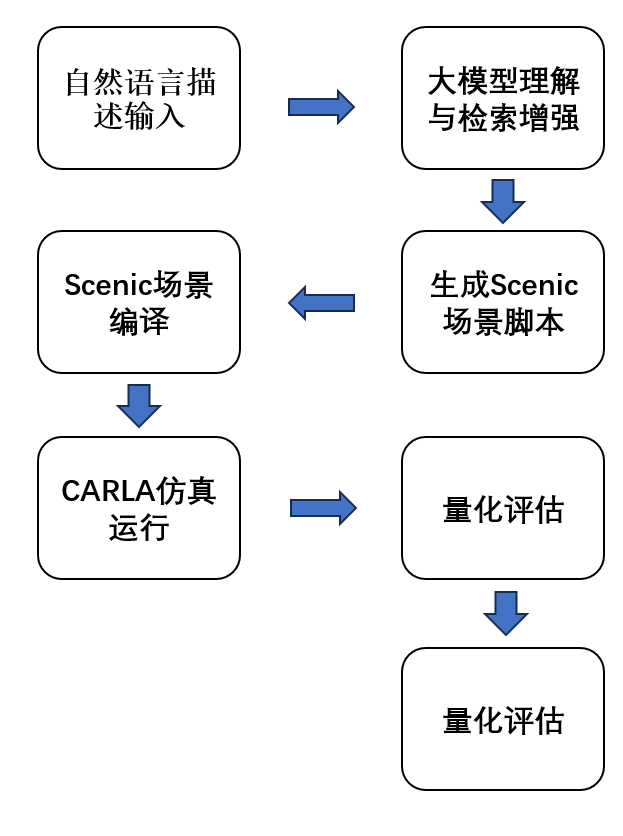
\includegraphics[width=0.9\textwidth]{../images/系统架构图.png} 
	\caption{系统架构图}
	\label{fig:system_architecture} % 添加合适的label
\end{figure}

\section{主要模块功能设计}
\subsection{自然语言理解与场景生成模块}
本模块负责接收自然语言输入并生成对应的Scenic场景描述。具体流程如下:
\begin{itemize}
	\item \textbf{输入}:自然语言形式的场景描述,例如“一个红色轿车在城市路口等待绿灯”。
	\item \textbf{检索增强}:使用 \texttt{sentence-transformers} 中的 \texttt{sentence-t5-large} 模型对输入进行向量化表示,并在本地检索数据库(如 \texttt{retrieve/scenario\_descriptions.txt})中查找相似描述作为参考样本。
	\item \textbf{大语言模型解析}:采用预训练的大语言模型(如 GPT-4o),结合检索到的参考样本,生成符合输入语义的 Scenic 脚本。
	\item \textbf{场景拼接机制}:根据场景复杂度,支持对多个子元素(如车辆、行人、环境条件)进行组织与拼接。
\end{itemize}


\subsection{场景合成与仿真模块}
本模块负责将生成的Scenic脚本转换为具体可运行的三维仿真环境。具体流程如下:
\begin{itemize}
	\item Scenic解析:调用Scenic的编译器,解析文本脚本,生成具体的场景配置,包括位置、速度、方向等参数。
	\item 仿真执行:通过CARLA仿真平台,依据Scenic配置文件动态构建三维场景,并设置相关仿真参数(如地图选择、天气条件、车辆行为模型等)。
	\item 接口调用关系:Scenic通过内部调用CARLA Python API,实现场景元素的部署与控制。
	\item 此模块支持动态场景生成,即支持车辆、行人在仿真过程中发生交互、运动与变化。
\end{itemize}

\subsection{场景评估与展示模块}
本模块负责对仿真完成后的场景进行可视化展示与量化评估。
\begin{itemize}
	\item 可视化展示:在仿真运行中自动截取场景关键帧截图或录制仿真过程视频,供人工审阅与验证。
	\item 量化评估:
	\begin{itemize}
		\item 语义保真度:通过人工或自动化对比,评估自然语言描述与实际生成场景之间的一致性。
		\item 多样性指标:统计不同输入自然语言生成场景在地图位置、交通元素种类、动态行为等方面的差异性。
		\item 驾驶性能指标:在生成场景中运行自动驾驶系统,评估其在仿真环境下的安全性(如碰撞率)、通过率(如成功驶出场景的比例)等指标。
	\end{itemize}
\end{itemize}